%!TEX program = xelatex
%\documentclass[cn,hazy,blue,14pt,screen]{elegantnote}
\documentclass{article}
\title{Latex笔记}

\author{姜嘉喆}
\date{\zhtoday}


\usepackage{ctex}  %中文出问题了用这个
%\usepackage{CJK} %中文出问题了用这个

%可能需要的:
\usepackage{amsmath}%数学公式
\usepackage{graphicx}%图片格式
\usepackage{amssymb}%特殊的数学符号
\usepackage{hyperref}%使用超链接
\usepackage{listings}%使用lstlisting
\usepackage{booktabs} %表格中要使用\toprule、\midrule、\bottomrule之类的命令需要用

\bibliographystyle{plain}%参考文献

\newtheorem{theorem}{Theorem}%以下四个是数学公式需要的环境
\newtheorem{lemma}{Lemma}
\newtheorem{proof}{Proof}[section]
\newtheorem{definition}{Definition}
\newtheorem{note}{Note}


\usepackage{graphicx} %插入图片的宏包
\usepackage{float} %设置图片浮动位置的宏包


\begin{document}
	
\maketitle

\graphicspath{{image}}
\begin{figure}[!htb]
\centering

\includegraphics[width=0.2\textwidth]{cat.png}
\end{figure}

\section{Latex安装}
其实可以在官网下载的,但我在软件管家公众号里下的,我下载的\href{https://mp.weixin.qq.com/s/PKXbMBmP8ounwbQE1OiRpw}{Latex2023},安装后长这个样子:
\begin{figure}[!htb]
\centering
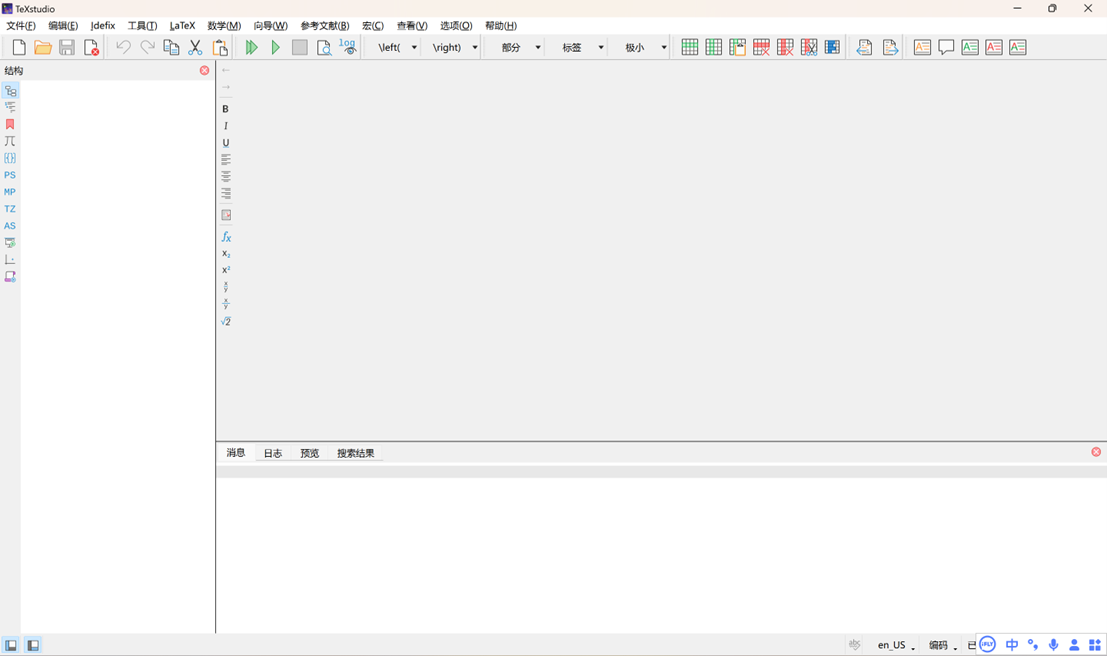
\includegraphics[width=0.9\textwidth]{image/Latex2023.png}
\end{figure}

\begin{note}
    安装步骤没问题也能用,但其实严格而言这个下载下来的桌面图像是texstudio编辑器,类比VS code编辑器;还有一个是Latex发行版,主要下载Tex Live。
\end{note}

\section{一些基本知识}
\href{https://mirrors.tuna.tsinghua.edu.cn/CTAN/info/lshort/chinese/lshort-zh-cn.pdf}{主要看的这本书}
补:有问题也可以问ChatGPT。。。。不仅能解决程序运行不出来的问题,提供的代码比你写的还简洁,效果还好。。。。。。。。。一个悲伤的故事


\begin{itemize}
	\item latex区分大小写,\verb|\LaTeX|,带*不带*
	\item 参数分为可选必选,[可选]\{必选\}
	\begin{lstlisting}
		\begin{环境名称}[可选参数]{必选参数}
			内容...
		\end{环境名称}
	\end{lstlisting}
	\item 在\verb|\documentclass|和\verb|\begin{document}|之间的位置称为导言区,在导言区中常会使用\verb|\usepackage| 命令调用宏包,还会进行文档的全局设置
	\item 在\verb|\documentclass[⟨options⟩]{⟨class-name⟩}|中,class-name为Latex提供的文档类,包含article(论文报告) report(综述长篇论文)nbook(书籍文档) proc(基于article的简单的学术文档模板) slides(ppt 使用无衬线字体) minimal(一个极其精简的文档类,只设定了纸张大小和基本字号,用作代码测
	试的最小工作示例) ;options可选择纸张大小基本字号排版方式对齐方式
	\item 可以用\verb|\input|命令插入文件,导言区或是复杂代码啥的
	\item 在导言区使用\verb|\syntaxonly|命令,可令LATEX 编译后不生成DVI或者PDF文档,只排查错误,编译速度会快不少
	\item 输入特殊字符需要用反斜线格式输入,\#之类的,输入\textbackslash 需要用\textbackslash
	\item \ldots 表示省略号,三个点;连字号- 用来组成复合词;短破折号– 用来连接数字表示范围;长破折号— 用来连接单词,语义上类似中文的破折号;重音字母或是其他特殊符号也有特殊指令
	\item 换行用\verb|\\|或\verb|\newline|,断页断词也有指令
	\item 不同类别的文档有不同的章节编号层级,可生成目录;文档结构划为前言正文后记,页码形式和编号变:\\
	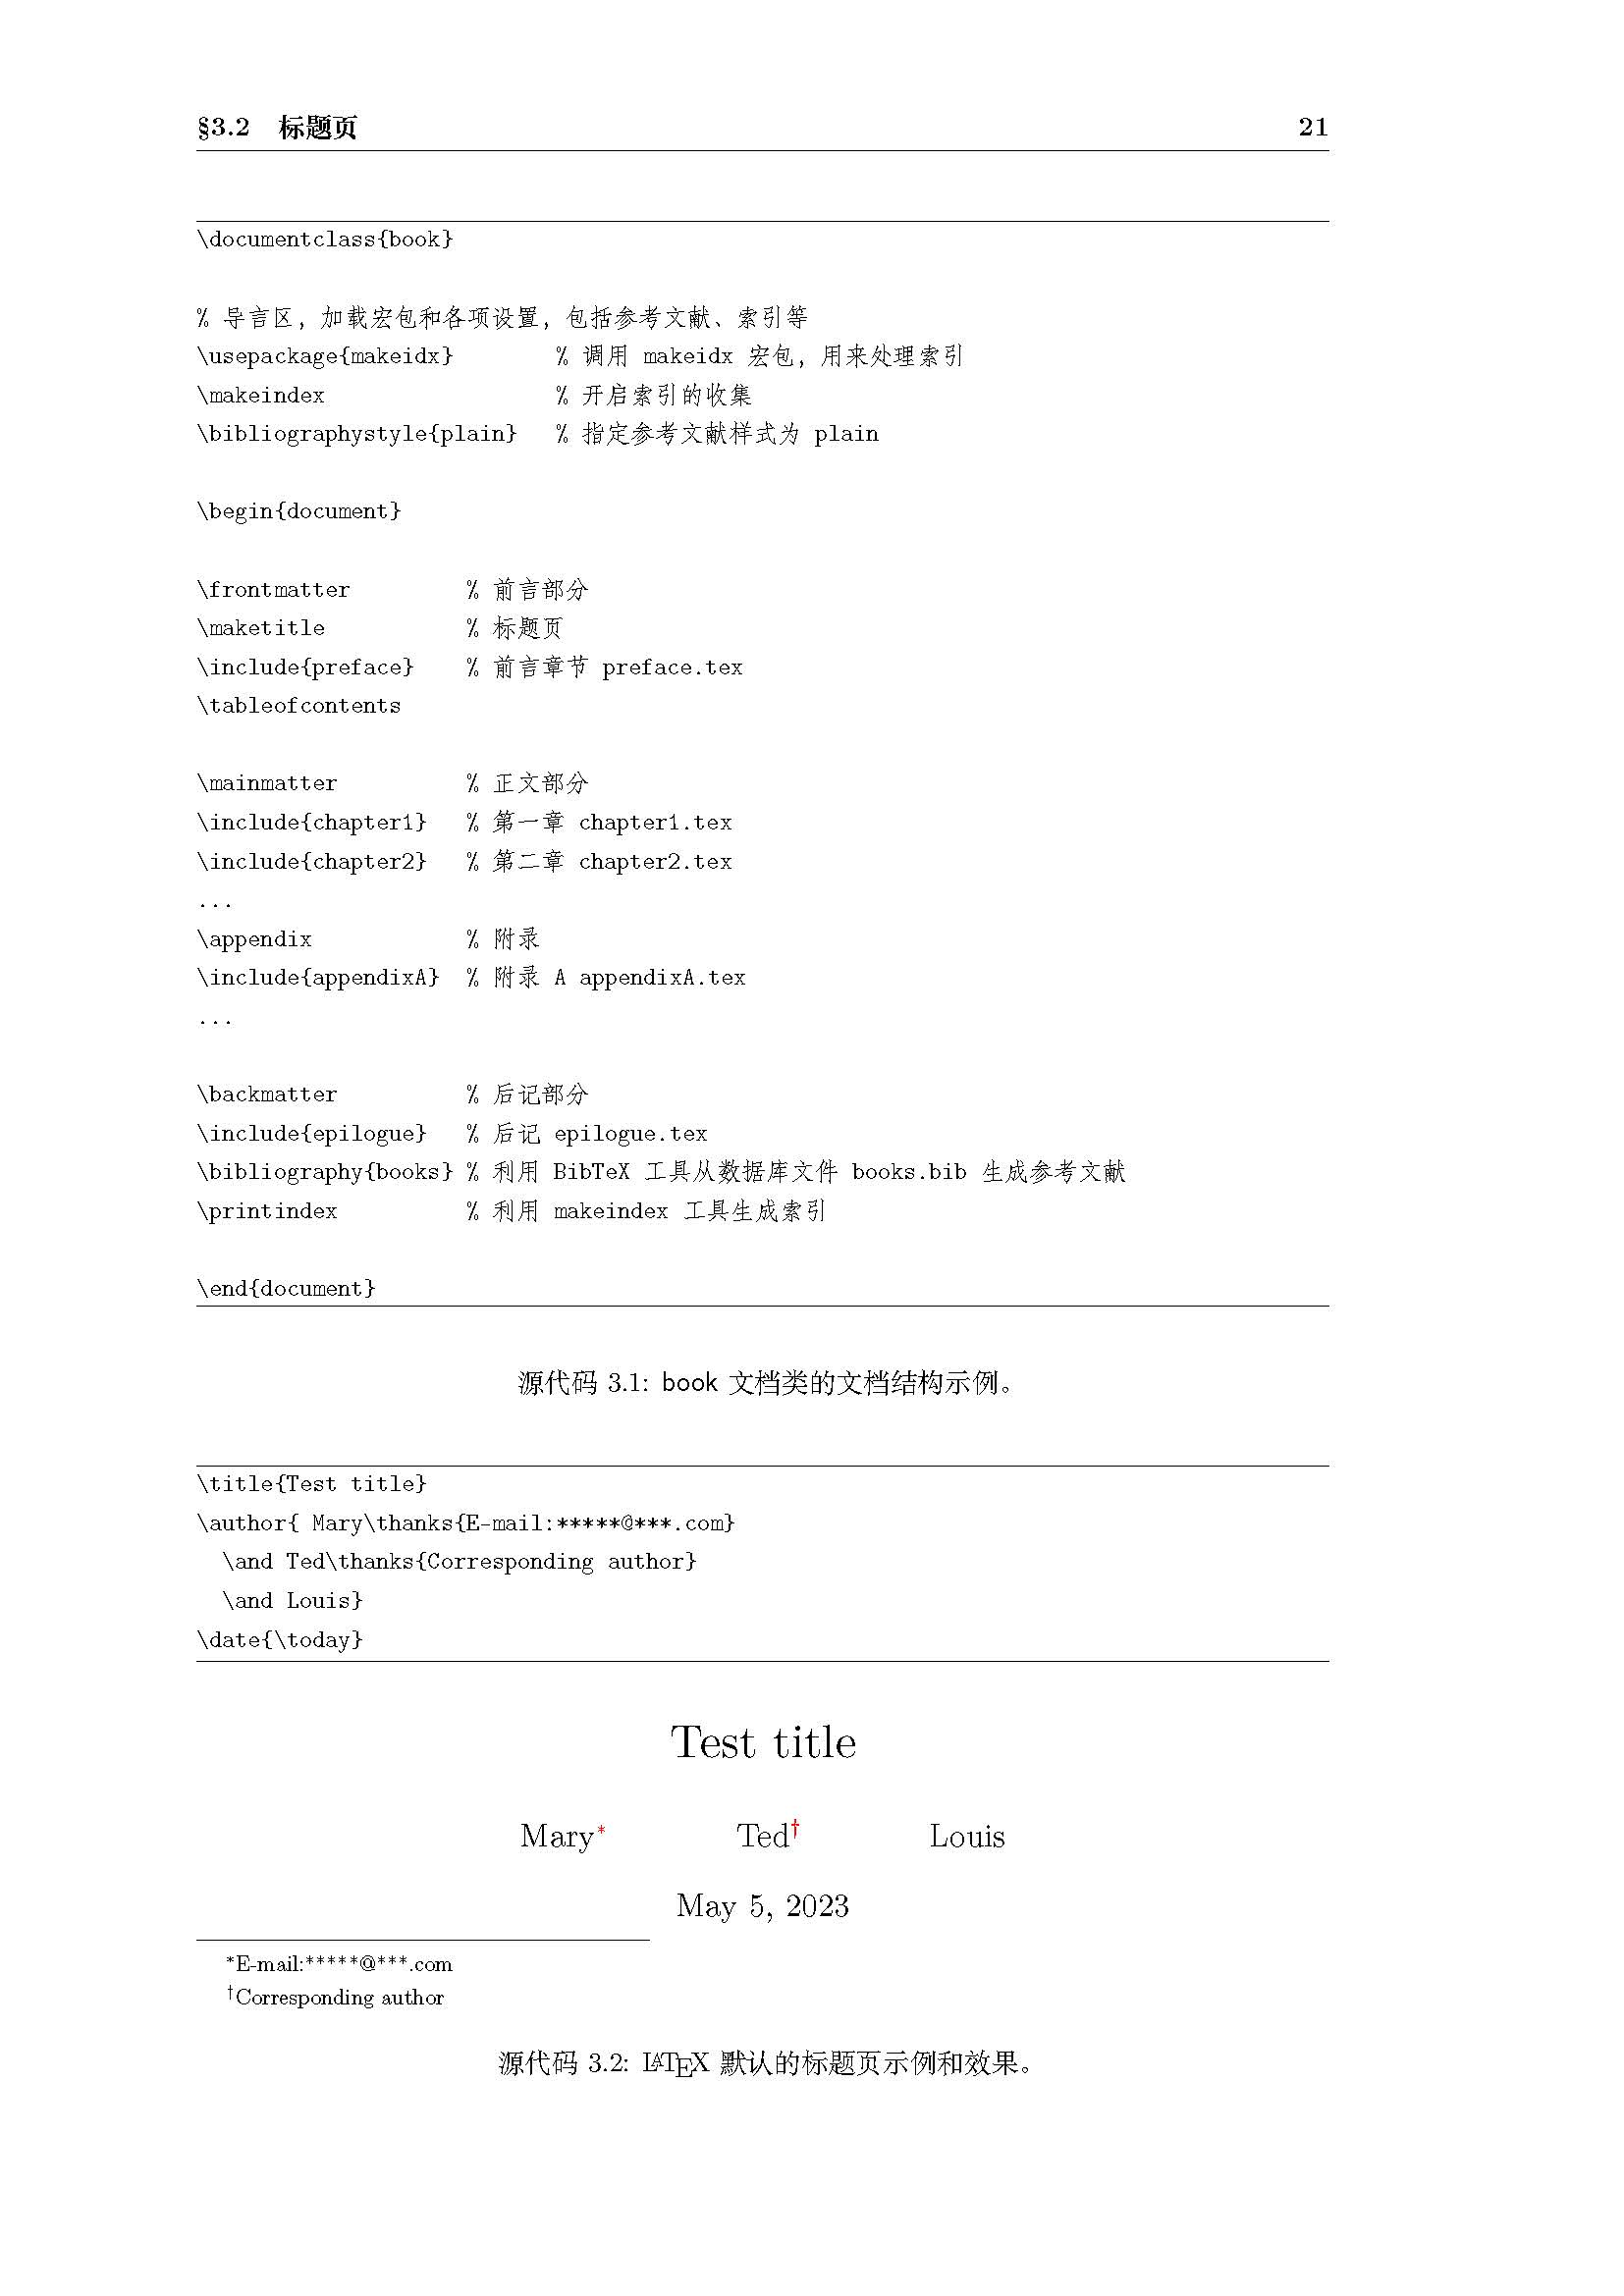
\includegraphics[width=\textwidth]{lshort-zh-cn_页面_033.jpg}
	\item 交叉引用:命名用\verb|\label{名字}|,引用用\verb|\ref{前面的名字}|或\verb|\pageref{前面的名字}|:see section ref\{名字\};脚注用\footnote{脚注},有些情况不能正确生成,到时候再看吧
	\item 对齐环境:center、flushleft 和flushright 环境分别用于生成居中、左对齐和右对齐的文本环境,begin\{center\}这么写;也可以直接用centering、raggedright、raggedleft指令,还有引用环境摘要环境代码环境(用begin\{verbatim\})(lstlisting)盒子啥的
	\item 浮动体:figure和table,习惯上figure里放图片,table里放表格,但并没有严格限制,可以在任何一个浮动体里放置文字、公式、表格、图片等等任意内容,位置参数[h][!h][b][!b][!t][t][p][!p]的含义:看图吧。。
	
	\begin{figure}[htbp]
		\centering
		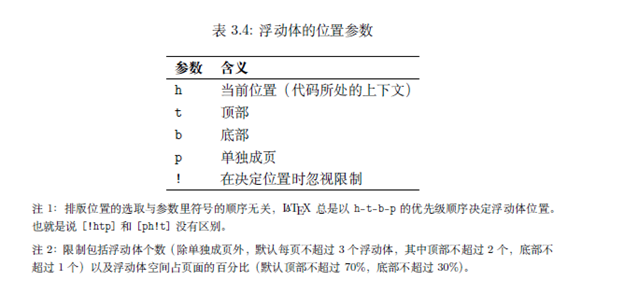
\includegraphics[width=\textwidth]{h.png}
		\caption{浮动体}
	\end{figure}


\end{itemize}




\section{如何插入部分}
(使用overleaf模板方法:在首页左上角New project——upload project,直接导入zip压缩文件)

可以用verb指令当引号用,但太麻烦了,反正真查的时候也是直接复制源代码里的东西的,索性直接写代码原样子了。加个\textbackslash 就行:

    插入图片格式:使用includegraphics[options]\{imagefile\}命令,比如这种的:[width=0.2\textbackslash textwidth]\{名字\},option里可以改变宽度高度大小啥的
    其他格式:让图片在begin\{figure\}下输入,可以用前面的对齐方式,end\{figure\}结束  

    插入网页链接格式:href{需要的链接}{你准备在文章里显示出的字}:

    插入代码格式:使用lstinline命令:
    
    直接lstinline{你要输的代码},或者使用begin{lstlisting}+end{lstlisting},中间是代码:

    插入脚注模式:{要标注的东西\footnote{脚注里要写的话}}

    插入图表模式:\ref{一个标签}
    
    这有个讲的更清楚的链接:\ref{几个数}
    
    https://blog.csdn.net/winycg/article/details/82633513

    还有个可以在线生成表格的网站:https://tablesgenerator.com
    \begin{table}[htbp]
    \centering% 显示位置为中间
    
    %\small
    \caption{我是第一个表的标题}
    \label{几个数}
    \begin{tabular}{lcc}% l代表左对齐,c代表居中,r代表右对齐
    \toprule
                  &     (1)    &      (2)      \\
    \midrule
    一个数         &    数值     &     数值     \\
                  &    (数值)   &     数值    \\
    两个数         &            &      数值   \\
                  &            &      (数值)   \\
    \bottomrule
    \end{tabular}%
  
\end{table}%

 这么写也行:(默认的)
 
 \begin{table}[htbp]
     \centering
     \begin{tabular}{c|c}
         1 & 2 \\
         3 & 4
     \end{tabular}
     \caption{我是第二个表的标题}
     \label{一个标签}
 \end{table}
    
\section{一些基本格式}
    插入不同类型的序号格式:3.1/(1)/1.2.3几种类型:

编号是需要计数器的,在标准的计数器中,只有roman、Roman、arabic、alph、Alph以及fnsymbol,其输出格式分别为i,ii、I,II、1,2、a,b、A,B、花体符号,使用
\begin{lstlisting}
  \renewcommand{\labelenumi}{\roman(变的地方){enumi}.} 
\end{lstlisting}
改变序号
    
\begin{enumerate}
\item arabic这种是1)的形式\\
    \begin{lstlisting}
      要写的东西,\啥的
    \end{lstlisting}
    
\end{enumerate}

\begin{itemize}  
    \item 这是点的模式,中间一个点
    \item 只有点无序号
\end{itemize}

\begin{description}
	\item[关键词] 和enumerate样子差不多,多个粗体关键词
	,
\end{description}
    
\subsection{这是直接3.1,3.2的格式}
  如果你想为自己的文档添加底色,可以在导言区添加下面设置:
  \begin{lstlisting}
    \definecolor{geyecolor}{RGB}{199,237,204}
    \pagecolor{geyecolor}
  \end{lstlisting}


\subsection{后面的接着写就行}
\begin{enumerate}
  \item 第一条
  \item 第二条
  \item 第三条
\end{enumerate}

也可以采取直接赋值的方法选择屏幕,比如:


\subsubsection{3.1.1的格式}
继续这么写



\section{数学符号部分}
导言区要\verb|\usepackage{amsmath}|
\href{https://zhuanlan.zhihu.com/p/464237097}{常用数学公式和符号}
\begin{enumerate}
	\item 公式有两种,行内公式用\verb|$$|包裹,行间公式用用begin\{equation\}环境,labei和ref交叉使用,eqref可自动加圆括号,tag修改公式编号名字,notag取消公式编号,别的方法如图所示:
	
\begin{figure}
\centering
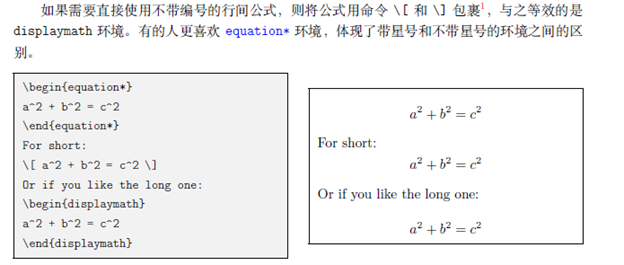
\includegraphics[width=\textwidth]{引用.png}
\caption{取消数学编号的其他方法}
\end{figure}

行内公式在排版大的公式元素(分式、巨算符等)时显得很“局促”

\item 数学模式中输入的空格被忽略,不允许有空行分段,所有的字母被当作数学公式中的变量处理,字母间距与文本模式不一致
\item 文档里(第41页)有一般符号、指数、上下标和导数、分式(是否为正常大小的)和根式、关系符(=<>)、算符(+-x)、巨算符(积分求和号)、数学重音和上下括号、箭头、括号和定界符、数组与矩阵(第47页)
\item 长公式折行:如果一定要折行的话,习惯上优先在等号之前折行,其次在加号、减号之前,再次在乘号、除号之前。其它位置应当避免折行,可以使用begin\{multline\} 书写折行长公式,它允许用\verb|\\| 折行,将公式编号放在最后一行。多行公式的首行左对齐,末行右对齐,其余行居中
\item 多行公式:align环境,它将公式用\&隔为两部分并对齐,分隔符通常放在等号左边,align环境会给每行公式都编号。我们仍然可以用notag去掉某行的编号;不需要等号对齐,用gather环境;公用编号,用aligned环境
\item 公式中的间距:挺多的,看图吧:

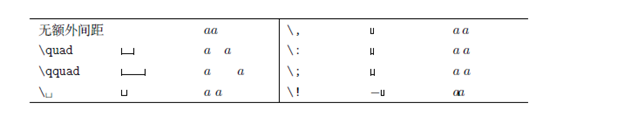
\includegraphics[width=\textwidth]{间距.png}

常见用于修正积分的被积函数$f(x)$ 和微元$dx$之间的距离
\item 也可以用usepackage{amssymb}切换部分符号字体,$\mathcal{R} \quad \mathfrak{R} \quad \mathbb{R}$之类的
\item 加粗用boldsymbol,也可指定选用行间公式行内公式
\item 定理环境:使用newtheorem环境定义定理名称格式,amsthm环境提供不带编号定理环境、证明环境(证毕符号)
\end{enumerate}

如果记笔记时不知道用哪个,直接在\href{https://www.latexlive.com/home##}{这里}截图识别图像并输入。

一个例子:

我们将通过三个步骤定义可测函数的积分。首先定义非负简单函数的积分。以下设 $E$ 是 $\mathcal{R}^n$ 中的可测集。

\begin{definition}[可积性]
设 $ f(x)=\sum\limits_{i=1}^{k} a_i \chi_{A_i}(x)$ 是 $E$ 上的非负简单函数,其中 $\{A_1,A_2,\ldots$, $A_k\}$ 是 $E$ 上的一个可测分割,$a_1,a_2,\ldots,a_k$ 是非负实数。定义 $f$ 在 $E$ 上的积分为 1. 3
\begin{equation}
   \label{inter}
   \int_{E} f dx = \sum_{i=1}^k a_i m(A_i).   \tag{使用tag自命标签}
\end{equation}
一般情况下 $0 \leq \int_{E} f dx \leq \infty$。若 $\int_{E} f dx < \infty$,则称 $f$ 在 $E$ 上可积。
\end{definition}

\begin{align}
	a & = b + c   \notag  \\
	& = d + e 
\end{align}

一个自然的问题是,Lebesgue 积分与我们所熟悉的 Riemann 积分有什么联系和区别?之后我们将详细讨论 Riemann 积分与 Lebesgue 积分的关系。这里只看一个简单的例子。设 $D(x)$ 是区间 $[0,1]$ 上的 Dirichlet 函数。即 $D(x)=\chi_{Q_0}(x)$,其中 $Q_0$ 表示 $[0,1]$ 中的有理数的全体。根据非负简单函数积分的定义,$D(x)$ 在 $[0,1]$ 上的 Lebesgue 积分为
\begin{equation}\label{inter2}
  \int_0^1 D(x)dx = \int_0^1 \chi_{Q_0} (x) dx = m(Q_0) = 0    \notag
\end{equation}
即 $D(x)$ 在 $[0,1]$ 上是 Lebesgue 可积的并且积分值为零。但 $D(x)$ 在 $[0,1]$ 上不是 Riemann 可积的。


\begin{theorem}[Fubini 定理]\label{thm:fubi}
若 $f(x,y)$ 是 $\mathcal{R}^p\times\mathcal{R}^q$ 上的非负可测函数,则对几乎处处的 $x\in \mathcal{R}^p$,$f(x,y)$ 作为 $y$ 的函数是 $\mathcal{R}^q$ 上的非负可测函数,$g(x)=\int_{\mathcal{R}^q}f(x,y) dy$ 是 $\mathcal{R}^p$ 上的非负可测函数。并且
\begin{equation}\label{eq:461}
  \int_{\mathcal{R}^p\times\mathcal{R}^q} f(x,y) dxdy=\int_{\mathcal{R}^p}\left(\int_{\mathcal{R}^q}f(x,y)dy\right)dx.
\end{equation}
\end{theorem}

\begin{proof}
Let $z$ be some element of $xH \cap yH$.  Then $z = xa$ for some $a \in H$, and $z = yb$ for some $b \in H$. Therefore $zH \subset xH$, as required.\cite{cn1}
\end{proof}


根据定理~\ref{thm:fubi},其运用十分广泛,可分为线性回归分析和非线性回归分析。\cite{cn2}

\section{排版样式设定}
可以自己设置字体(样式)和字号(大小)、文字的下划线、通过一堆长度变量控制版面格式,如页面宽度和高度、首行缩进、段落间
距等、行距(可直接在导言区设置或局部改变)、段落格式(左缩进、右缩进和首行缩进)、水平垂直间距、页面与分栏、页眉页脚

\section{参考文献使用}

本来写了挺多的,但想了想,用的时候直接复制吧,毕竟参考文献格式都是直接复制的,本文用的BibTeX格式(其实也有其他的,但就用这个吧)

参考文献格式:
\begin{lstlisting}
	@book{renardy2006introduction,
		title={An introduction to partial differential equations},
		author={Renardy, Michael and Rogers, Robert C},
		volume={13},
		year={2006},
		publisher={Springer Science \& Business Media}
	}
\end{lstlisting}
我举的这个例子中,第一行renardy2006introduction是索引名字,可以改成另外一个,cn1啥的,引用时用cite\{cn1\}

BIBTEX程序在生成参考文献列表的时候,通常只列出用了\verb|\cite| 命令引用的那些,或者:

\begin{lstlisting}
	\nocite{⟨citation⟩}%列出未被引用的文献
	\nocite{*}%所有未被引用的文献都列出
\end{lstlisting}

引用参考文献格式:
\begin{enumerate}
\item 准备一份BIBTEX 数据库,假设数据库文件名为books.bib,和LATEX 源代码一般
位于同一个目录下。	
\item 在源代码中添加必要的命令。假设源代码名为demo.tex,利用books.bib 生成参考文献的源代码demo.tex:
\begin{lstlisting}
	\documentclass{article}
	\bibliographystyle{plain}
	\begin{document}
	\section{Some words}
		Some excellent books, for example, 
		\cite{参考文献1} and \cite{参考文献2} \ldots
	\bibliography{books}
	\end{document}
\end{lstlisting}
注意:bibliographystyle 和bibliography 命令缺一不可,没有这两个命令,使用BIBTEX生成参考文献列表的时候会报错.
\item 还有添加PDF书签、改变文档属性啥的,用到再说吧
\end{enumerate}

\section{绘图功能}
使用tikz宏包绘图,用直角坐标系或极坐标描述点的位置,可画一些常见图形及抛物线。也可填充颜色指定线条类型文字结点循环啥的,等用到的时候再说吧。再说了,麻烦的图直接通过其他软件生成*.eps图片再插入,不是更好吗。。。

\section{制作ppt}
这有一本汉化过的三百多页的beam包使用说明书。。。
\href{http://static.latexstudio.net/wp-content/uploads/2017/02/BeamerUserGuide_V3.24_zh-cn.pdf}{用户手册}


使用beamer环境,一帧是一页,用frame,也可以直接在后面加\{\}:
\begin{lstlisting}
\begin{frame}{古数学}{定理发现}
	发现了一些定理
		
	比如说:
\begin{itemize}
	\item 公元前11世纪
	\begin{quote}      %是一页帧,但点一下出一点,这块的代码实际上有四页
		勾三股四玄五
	\end{quote}
	\item 又比如说
	\begin{quote}
		$3^2+4^2=5^2$
	\end{quote}
\end{itemize}
end{frame}	
\end{lstlisting}

样子长这样:

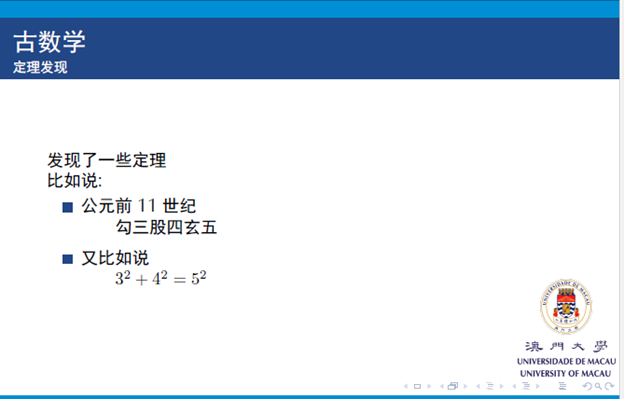
\includegraphics[width=\textwidth]{ppt1.png}

开始会使用\verb|\usetheme{Berlin}|指定ppt的主题包,berlin是其中一种。全部主题包及示例可以看\href{https://blog.csdn.net/zhouxiaowei1120/article/details/82818295}{这里};可以使用\verb|\usecolortheme{lily}|指定ppt的主题颜色,全部主题颜色及示例可以看\href{https://blog.csdn.net/zhouxiaowei1120/article/details/82818348?spm=1001.2014.3001.5502}{这里}

使得每个章节都有小目录:
\begin{lstlisting}
\AtBeginSection[]
{
	\begin{frame}<beamer>
		\frametitle{\textbf{目录}}
		\tableofcontents[currentsection]
	\end{frame}
}
\end{lstlisting}

可以使用columns环境分栏,一般把图片放在左侧;插入网页可以使用这种形式:

\begin{lstlisting}
\begin{block}{代码地址}
	\url{https://github.com/aipuxilong0618/pde_note}
\end{block}
\end{lstlisting}

另:\lstinline|\begin{column}<0->{.5\textwidth}|含义:该列从幻灯片放映的开头开始显示其内容,并占据幻灯片上可用宽度的 50%。

另:选取部分主题后转成ppt后所有的block都会变成黑框。。神奇,最后我用的默认default的

\section{一些其他问题}
\begin{enumerate}
  \item \textit{如何忽视TeX命令原样输出其中的文本?}\\
    使用\verb|\verb|命令,\:\verb|verb||你准备引用的东西|;
    
    也可以使用\verb|\lstinline|命令,只是\verb|\lstinline|输出的是代码格式,
    如\verb|\lstinline{你要输的代码}|,可能会呈现出不同的颜色,\lstinline{\author}与\verb|\author|的区别
    
  \item \textit{警告问题}\\
    显示\verb|Overfull \hbox|问题,该异常多是由于LaTeX找不出断句处单词的连字符位置,从而不能正常断句,\href{https://zhuanlan.zhihu.com/p/131667648}{看这个}
    
    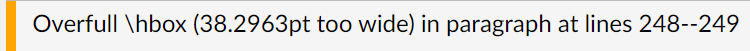
\includegraphics[width=0.8\textwidth]{image/over.png}
%   \item \textit{颜色变幻}\\  
%     模板中一共有5套颜色主题,分别是:\textcolor{eblue}{blue}(默认)、\textcolor{egreen}{green}、\textcolor{ecyan}{cyan}、 \textcolor{sakura}{sakura} 和\textcolor{black}{black}。
   
\end{enumerate}

\bibliography{reference}
%\nocite{*}%引用bib文档中的全部参考文献
%\printbibliography[heading=bibintoc, title=\ebibname]
%\bibliography{reference}
%\bibliographystyle{}
\end{document}
